\chapter{Conclusions and Future Work}
\label{ch:ConclusionFutureWork}

% --------------------------------------------------------
% Restating to the thesis
% --------------------------------------------------------

Load balancing is a classic problem in HPC, which largely depends on a specific context and an imbalance cause. Our work focuses on the imbalance of task-based parallel applications when running in distributed memory systems. \\

The context can be determined when our application has a number of compute tasks assigned to typical execution units called processes. With today's multicore computing architectures and task-based parallel programming models, a process can be mapped to a multicore processor, in which we can create multiple threads mapped to cores where tasks are executed.\\

Regarding the imbalance, the main cause is performance slowdown that occurs on some processes, causing a slower execution than usual. Moving tasks from slow to fast processes is the only way to balance the load. However, the challenge is communication overhead since task migration is costly. This requires an appropriate approach to migrate as many tasks as appropriate from/to a potential process.\\

% --------------------------------------------------------
% Summarize key points
% --------------------------------------------------------

Through the research process, we obtained some key points:
\begin{itemize}
	\item The classic approach suitable for our context is work stealing, which is widely studied in shared memory systems. However, communication in distributed memory systems hinders this approach because stealing a task can be time-consuming. Therefore, communication overhead can limit the number of tasks that can be stolen.
	
	\item An improvement of work stealing in distributed memory is reactive load balancing, which is a state-of-the-art approach. Reactive load balancing leverages task-based programming models and multicore architectures to perform reactive task migration. Unlike the pull-oriented mechanism of work stealing, the reactive approach uses a dedicated thread in each process to continuously check the execution status. Following that, we can speculatively detect an imbalance earlier, and tasks can be migrated earlier. However, this approach is quite risky in the case of high imbalance because reactive task migration is only based on the most current execution status at a time and is quite speculative. The number of times migrating incorrect tasks can occur frequently in some cases, such as when the number of tasks is large and the load difference is high.
	
	\item The factors affecting dynamic load balancing include both application and system characteristics. In particular, an application can be characterized through the number of tasks, execution scale (e.g., the number of compute nodes and processes), data size of tasks. The system's characteristics include communication overhead, performance variability.
	
	\item Both work stealing and reactive load balancing can be slow at runtime due to their characteristics. For instance, work stealing starts stealing tasks when one of the processes is idle, while reactive load balancing operations are quite speculative.
	
	\item An important point about dynamic load balancing in general and about our context in particular is the lack of load information. This is understandable since most current approaches are based on little information, such as the execution status inferred from the queue length of each process.
\end{itemize}

% --------------------------------------------------------
% Highlight implications and contributions
% --------------------------------------------------------

The key points above motivate our contributions, including:
\begin{enumerate}
	\item A new performance model: We show that an appropriate performance model is essential to analyze the operations and limitations of the current approaches.
	\item A new proactive load balancing approach: We show a new idea called ``proactive load balancing'', where the load knowledge can be generated at runtime through online load prediction.
\end{enumerate}

Our model is based on discrete-time modeling towards simulating reactive load balancing behavior through the operations, such as monitoring execution status, exchanging status, checking imbalance, and offloading tasks. These are continuously and spontaneously performed at runtime. To facilitate analyzing the performance model, we combine:
\begin{itemize}
	\item the operations of monitoring, exchanging, and checking into a balancing cost parameter, which implies an average cost of balancing operations.
	\item the operations of offloading tasks into a task migration cost parameter, which is affected by delay time in distributed memory.
\end{itemize}

Most previous performance models typically focus on the task migration cost parameter because transmission time in distributed memory systems is high. However, our proposed model shows that the cost of balancing operations also keeps a high impact. Although each operation costs insignificantly, a large number of operations can produce a large impact. When the number of tasks and the imbalance are high, these balancing operations lead to large delays before a task can be migrated.\\

Work stealing and reactive load balancing work without prior knowledge at runtime; hence, the balancing operations are performed continuously and repeatedly. Only relying on the execution status at a certain time to decide task migration is not enough. This perspective motivates our proactive approach. The load prediction helps determine imbalance levels, which processes are overloaded and underloaded. Following that, we can better estimate the number of tasks that should be migrated. We confirm the benefits of proactive load balancing through two methods:
\begin{itemize}
	\item Feedback task offloading
	\item ML-based task offloading
\end{itemize}

Our implementation is designed as a plugin tool of a task-based programming framework named Chameleon. Through the experiments on microbenchmarks and a real application called Sam(oa)$^2$, we show a speedup improvement on average between $1.7\times$ - $3.5\times$ in significant imbalance cases.\\

Furthermore, our approach supports a new idea: co-scheduling tasks across multiple applications. The scope of scheduling tasks is not only in a single application but also in multiple applications running simultaneously. We can share tasks across multiple applications to make them better in using resources and balancing load.\\

Nevertheless, our work has limitations related to the proposed performance model and the proactive load balancing approach. This implies future research directions that are shown in the following part.\\

% --------------------------------------------------------
% Limitations and Future Works
% --------------------------------------------------------
% \noindent \textbf{Future Work} \\

\begin{figure}[ht]
  \centering
  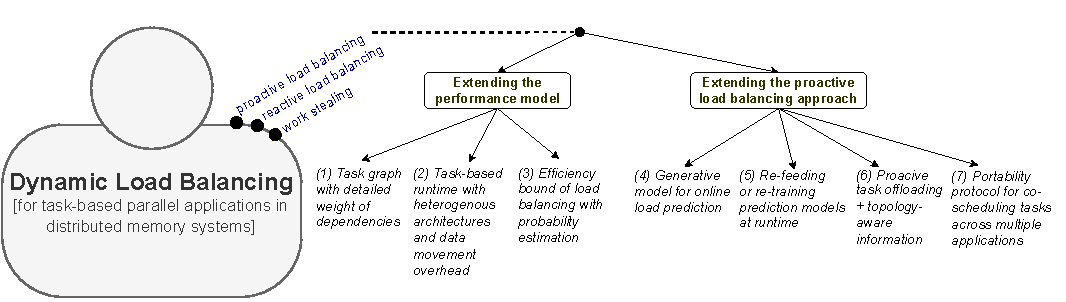
\includegraphics[scale=0.85]{./pictures/future_work/future_work_overview.pdf}
	\caption{An overview of future work for further research directions.}
	\label{fig:future_work_overview}
\end{figure}

In the future, the following potential work can be considered. Figure \ref{fig:future_work_overview} shows seven research directions based on two branches:

\begin{itemize}
	\item Extending the performance model: Our model revolves around the influence parameters, including the number of tasks ($T$), processes ($P$), performance slowdown factor ($Slow$), execution speed of a process ($S_{P}$), overhead in balancing operations ($O_{\text{balancing}}$), and delay time in task migration ($d$). However, other factors and aspects should be oriented in the future, following the sub-branches (1), (2), (3).
	\item Extending the proactive load balancing approach: Our approach exploits one core in a multicore processor to dedicate a thread for communication and load balancing. When this thread can be used to perform different things at runtime, such as load prediction and communication between different applications running at the same time, then we can improve it following the sub-branches (4), (5), (6), (7).
\end{itemize}

The details of each sub-branch are as follows:

% -------------------------------------------------
% Branch 1: theory side with a performance model
% -------------------------------------------------

\begin{enumerate}[label=(\arabic*)]
	\item Task-based applications with dependencies: implies a graph of tasks. Assuming the edges in the graph represent waiting time (weight) among tasks, the effect of these weights is challenging task migration for dynamic load balancing.
	\item System with heterogeneous architectures: implies the problem of modeling heterogeneous tasks and different communication overhead in task migration.
	\item Using probability to estimate the limit of task migration in reactive and proactive load balancing: implies a mathematical proof based on probability to analyze the limit of task migration.

% -------------------------------------------------
% Branch 2: proactive load balancing
% -------------------------------------------------

%\begin{enumerate}[label=(\arabic*)]
%	\setcounter{enumi}{3}
	\item Generative model for online load prediction: indicates a generative model for predicting load automatically. A generative model can reduce user's effort in guiding and collecting influence features at runtime.
	\item Re-feeding and re-training prediction model at runtime: indicates the methods that we can use to perform auto-feeding and auto-training for online load prediction.
	\item Proactive load balancing + topology information: indicates an integration of topology information with proactive task offloading. ``Proactive'' provides an appropriate number of tasks and processes to perform task migration. However, if the knowledge of hardware topology can support information about which process is fast in communication, then we can improve migration strategies further.
	\item Portability for co-scheduling tasks across multiple applications: indicates a generalized protocol in distributed memory systems, which supports enabling co-scheduling tasks in a simplified method.
\end{enumerate}

% --------------------------------------------------------
% Ending on a strong note
% --------------------------------------------------------

All in all, we conclude that optimizing dynamic load balancing in distributed systems requires consideration between strategy and time. Strategy concerns passive and active, operations and their cost, while time is associated with tasks and the cost of migrating tasks. With current computing architectures and new programming models, such as task-based programming, our approach shows feasibility and efficiency. In particular, we leverage machine learning as a load-balancing support tool. For a long-term vision, this work is compatible with automatic tuning as well as automatic scheduling for high-performance applications based on human rules and policies.

% We conclude two observations around dynamic load balancing with task-based parallel applications that are deployed on distributed memory systems. First, a specific context characterized from both application and system determines load balancing performance, including the number of tasks, the scale of processes/nodes, the data size of tasks, and the characteristics of distributed memory, such as communication overhead and performance variability. Second, the traditional and current approaches, i.e., work stealing and reactive load balancing, may be too late in terms of migrating tasks for load balancing.\\

% The behavior of work stealing is considered passive because tasks are stolen from a busy process only when existing an idle process. Stealing operations can be delayed and missed due to latency and transmission time. The current approach known as an improvement is reactive load balancing, in which we attempt to offload tasks earlier instead of stealing. The idea is based on execution scheme of task-based programming models, where we separate the control between tasks and computing resources (denoted by executing-tasks threads per process). Tasks are scheduled into a pool of threads, in which one thread is dedicated ($Tcomm$) to perform load balancing. In reactive load balancing, $Tcomm$ is deployed to monitor the execution speed of each process and exchange this information around. Based on the information, we can determine slow processes, fast processes, and offload tasks earlier. However, we observe that the reactive approach might take late as well as incorrect decisions in high imbalance scenarios.\\

% This thesis first contributes a performance model to analyze the limit of reactive load balancing. We classify two types of overhead before a task is offloaded, one by balancing operations in general and one by task migration delay. With balancing operations, the overhead of each might be trivial, but reactive approach (or even work stealing) do not perform only a few of them at runtime. Therefore, many operations of reactive load balancing can be limited due to speculative decisions in offloading tasks. Especially, the most current status driving the decision of reactive task offloading is insufficient. Our model formulates and addresses this limit through different influence parameters such as the number of tasks ($T$), processes ($P$), imbalance ratio ($R_{imb}$), performance slowdown factor ($Slow$), latency ($\lambda$), and task migration delay ($d$). \\

% Following that, we second contribute a new approach called proactive load balancing. The approach is developed toward proactive task offloading methods upon a task-based programming model. We exploit $Tcomm$ to generate knowledge about runtime load values instead of only speculatively monitoring the queue length to decide offloading tasks. In our approach, $Tcomm$ is dedicated to task characterization, online load prediction, and proactive task offloading. With load information at runtime, we can estimate how many tasks should be offloaded at once and which processes are suitable to migrate them. These points motivate us to propose two methods upon the approach: feedback task offloading and ML-based task offloading.\\

% For proof of concept, we introduce a simulator and a reference implementation addressed as a plugin tool upon a given task-based programming framework named Chameleon. We evaluate performance by using micro-benchmarks and a realistic use case called Sam(oa)$^2$. Sam(oa)$^2$, known as a scientific computing simulation in HPC, mainly supports oceanic applications developed via the concept of adaptive mesh refinement and space-filling curves. All experiments are performed in three different clusters. Our results confirm the benefits in high imbalance cases, gaining around $1.7\times$ - $3.5\times$ compared to reactive load balancing and randomized work stealing. As an extension, this approach opens a new method for co-scheduling tasks across multiple applications such a long-term vision.

% In HPC clusters, resources indicates compute nodes, one node today includes several multicore processors. When a task-based programming runtime map the execution of tasks on one process

% First, the proposed performance model aims at reactive load balancing as well as work stealing under the overhead of balancing operations and delay time in task migration. It revolves around the influence parameters, including the number of tasks ($T$), processes ($P$), performance slowdown factor ($Slow$) (or execution speed per process, $S_{P}$), overhead in balancing operations ($O_{\text{balancing}}$), and delay time ($d$). Our performance model generally attempts to estimate the limit of dynamic load balancing. We target how far a balancing method can reduce the imbalance level denoted by $R_{imb}$ as well as completion time through the number of migrated tasks. However, other factors and aspects should still be oriented in the future as follows.

% Second, proactive load balancing opens further directions toward co-scheduling tasks across multiple parallel applications. Our scheme dedicates one-core-off to control proactive load balancing, which can be considered as a talking channel between different applications that are run simultaneously. Some further research directions following this scheme can be addressed as follows.

%
%\section{Conclusions From Question Q3:}
%\paragraph{Q3:
%\begin{enumerate}[label=Q\arabic*]
%        \setcounter{enumi}{2}
%    \item --
%        How can such a model be applied to concrete system architectures for \pne management of \glspl*{HPC system}?}
        %%% ANSWER: A guide to create concrete instances of the \gls*{OIEPrefmodel}, named \glspl*{OIEParch}.
%\end{enumerate}
%Conclusions:
%\begin{itemize}
%    \item To answer Question~3, a method for the application of the reference model is needed.
%        Such method is constructed and presented in Section~\ref{sec:Arch-Method}.
%    \item The method is tailored towards applying the \gls*{OIEPrefmodel} for the construction of \glspl*{OIEParch}.
%\end{itemize}
%
%\begin{itemize}
%    \item To model existing \glspl*{HPC system} using the \gls*{OIEPrefmodel}
%        and construct \glspl*{OIEParch} for them, their structure has to be analyzed.
%    \item The identified components then have to be mapped to the building blocks provided by the reference model.
%    \item The result is a transparent and understandable model of the \pne management system for a given \gls*{HPC system}.
%    \item This process is applied and its feasibility shown.
%\end{itemize}
%With the conclusions from Questions Q2 and~Q3, the solution to Question~Q1 is
%supplemented and finalized.
%The method followed in this work is concluded and the contributions fulfilled.
%

%~\\\\
%\paragraph{Concluding Remark}
%~\\\\
%With the presentation of the contributions and the conclusions to the problem
%statement and research questions, the overall problem statement is satisified.
%This work is a stepping stone towards modeling \pne management systems of
%\glspl*{HPC system}, by providing the first \gls*{ReferenceModel} for describing
%hierarchical \pne management system for \glspl*{HPC system}:
%the \acrfull*{OIEP} \glslink*{OIEPrefmodel}{reference model}.
%END OF WORK
